\documentclass[tikz,border=3pt]{standalone}
\usepackage{lmodern}
\usepackage{xcolor}
\usetikzlibrary{arrows.meta}


\begin{document}
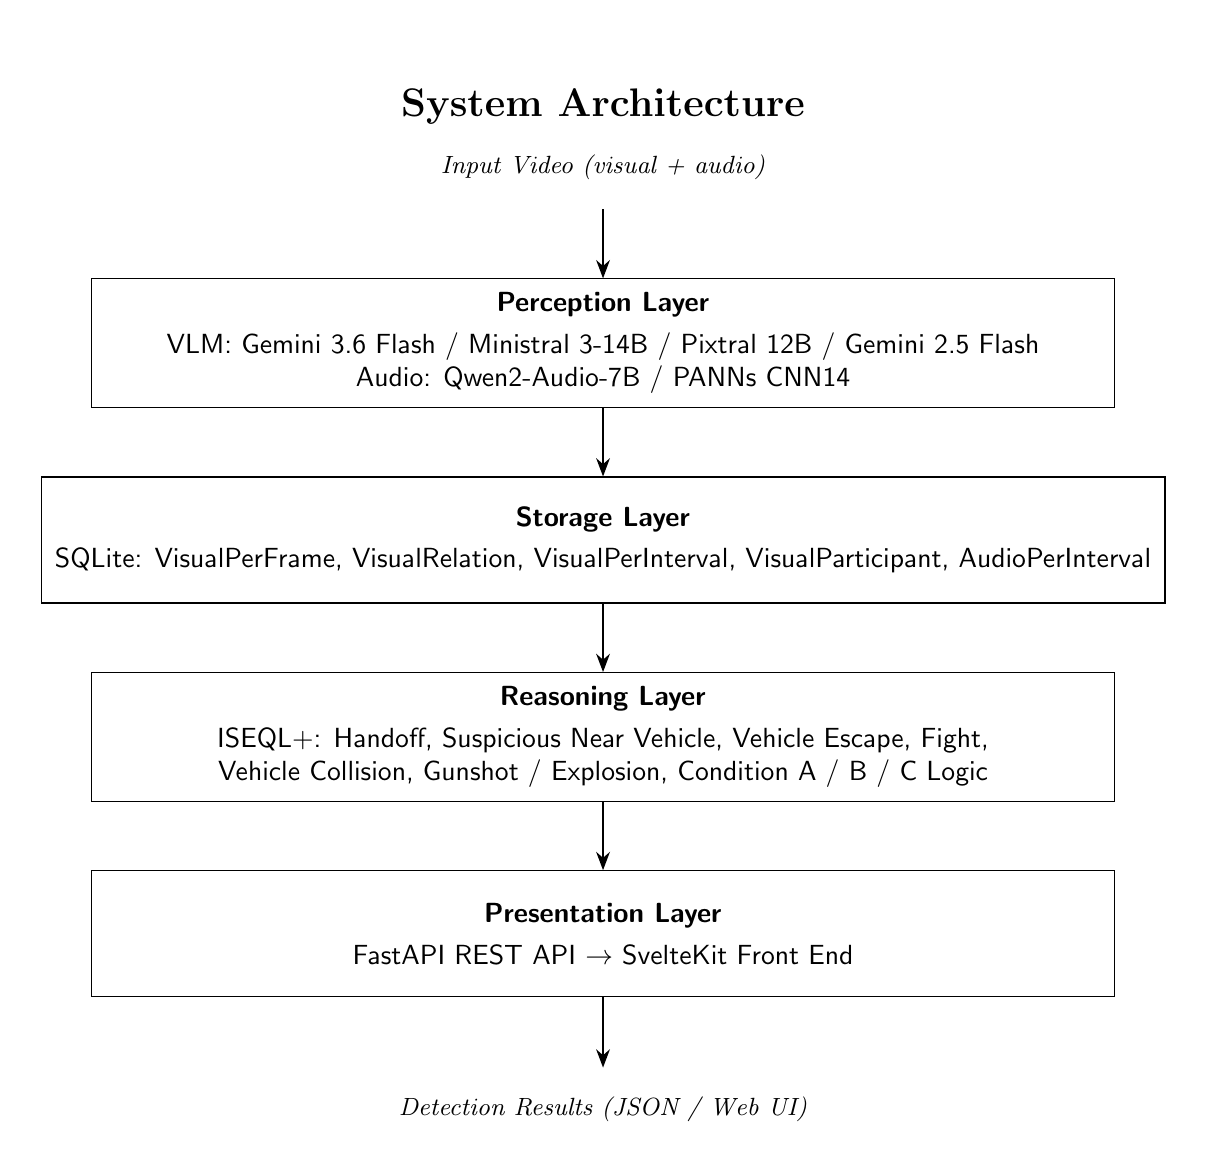
\begin{tikzpicture}[
  every node/.style={font=\sffamily},
  box/.style={draw=black, align=center, inner sep=5pt, minimum height=1.6cm},
  note/.style={font=\small\itshape, align=center},
  arrow/.style={-Stealth, thick},
]

\draw[white] (-0.3,-0.5) rectangle (14.3,12.5);

\node[font=\Large\bfseries] at (7,11.5) {System Architecture};

\node[box,fill=white, minimum width=13cm] (L4) at (7,8.5) {
    \textbf{Perception Layer}\\[3pt]
    VLM: Gemini 3.6 Flash / Ministral 3-14B / Pixtral 12B / Gemini 2.5 Flash\\
    Audio: Qwen2-Audio-7B / PANNs CNN14
};

% Input at top
\draw[arrow] (7,10.2) -- (L4.north);
\node[note, anchor=south] at (7,10.45) {Input Video (visual + audio)};

\node[box,fill=white, minimum width=13cm] (L3) at (7,6.0) {
    \textbf{Storage Layer}\\[3pt]
    SQLite: VisualPerFrame, VisualRelation, VisualPerInterval, VisualParticipant, AudioPerInterval
};

\node[box,fill=white, minimum width=13cm] (L2) at (7,3.5) {
    \textbf{Reasoning Layer}\\[3pt]
    ISEQL+: Handoff, Suspicious Near Vehicle, Vehicle Escape, Fight,\\
    Vehicle Collision, Gunshot / Explosion, Condition A / B / C Logic
};

\node[box,fill=white, minimum width=13cm] (L1) at (7,1.0) {
    \textbf{Presentation Layer}\\[3pt]
    FastAPI REST API $\rightarrow$ SvelteKit Front End
};

\draw[arrow] (L4.south) -- (L3.north);
\draw[arrow] (L3.south) -- (L2.north);
\draw[arrow] (L2.south) -- (L1.north);

% Output at bottom
\draw[arrow] (L1.south) -- (7,-0.7);
\node[note, anchor=north] at (7,-0.95) {Detection Results (JSON / Web UI)};

\end{tikzpicture}
\end{document}
